\documentclass[presentation]{beamer}
\usepackage{../oop-slides-pianini}
\usepackage{url}
\setbeamertemplate{bibliography item}[text]

\title[Code quality]{06\\ Qualità del codice, librerie, programmazione multipiattaforma, deployment, profiling}

\begin{document}

\frame[label=coverpage]{\titlepage}

\section{Preparazione al laboratorio}

\begin{frame}{Preparazione dell'ambiente di lavoro}
	\begin{enumerate}
		\item Clonare il repository degli esercizi
		\begin{itemize}
            \item Opzionalmente, si fork-i il repository
		\end{itemize}
		\item Importare il repository in Eclipse come progetto Java
		\begin{enumerate}
			\item File
			\item Import
			\item General
			\item Existing project into workspace
			\item Si selezioni la cartella del progetto
			\item Si confermi l'import
		\end{enumerate}
		\item \alert{Configurare correttamente Eclipse, abilitare e configurare i plugin per il controllo di qualità del codice}
	\end{enumerate}
\end{frame}

\begin{frame}{Modalità di lavoro}
	\begin{enumerate}
		\item Seguire le istruzioni del file README.md nella root del repository
		\item Tentare di capire l'esercizio in autonomia
		\begin{itemize}
			\item Contattare il docente se qualcosa non è chiaro
		\end{itemize}
		\item Risolvere l'esercizio in autonomia
		\begin{itemize}
			\item Contattare il docente se si rimane bloccati
		\end{itemize}
		\item Utilizzare le funzioni di test per verificare la soluzione realizzata
		\item Cercare di risolvere autonomamente eventuali piccoli problemi che possono verificarsi durante lo svolgimento degli esercizi
		\begin{itemize}
			\item Contattare il docente se, anche \textbf{dopo aver usato il debugger}, non si è riusciti a risalire all'origine del problema
		\end{itemize}
		\item Scrivere la Javadoc per l'esercizio svolto
		\item \alert{Assicurarsi che non ci siano warning nel proprio codice}
		\item Effettuare \textit{almeno} un commit ad esercizio completato
		\item \textbf{A esercizio ultimato sottoporre la soluzione al docente}
		\item Proseguire con l'esercizio seguente
	\end{enumerate}
\end{frame}

\section{Programmazione multipiattaforma}

\begin{frame}{``Write once, run anywhere...''}
	Lo slogan coniato originariamente da Sun Microsystems per illustrare i benefici del linguaggio Java vale a patto che:
	\begin{enumerate}\itemsep10pt
		\item \textbf{``write'' sia fatta in modo corretto e robusto},
		\begin{itemize}
			\item ovvero, sia adottato un approccio di programmazione adeguato.
		\end{itemize}
			\item \textbf{sia possibile distribuire ciascuna applicazione per qualunque piattaforma}.
		\begin{itemize}
			\item ovvero, sia predisposto un deployment efficace. 
		\end{itemize}
	\end{enumerate}
\end{frame}

\subsection{Accesso al file system}

\begin{frame}{Path e Separatori}
	Inserire dei path assoluti nel proprio sorgente è \textbf{sempre} fonte di problemi quando si scrive software multipiattaforma:
	\begin{itemize}
		\item \url{C:\\Users\\UserName\\file} --- Non funzionerà su piattaforma *nix, e non funzionerà se l'utente Windows non è ``UserName''.
		\item \url{C:\\MyProgram\\file} --- Non funzionerà su piattaforma *nix, e non funzionerà se 
l'installazione di Windows è sana e il software non è avviato con diritti di amministratore.
		\item \url{/home/username/file} --- Non funzionerà su piattaforma Windows, e non funzionerà se l'utente non è \texttt{username}.
	\end{itemize}
	\begin{block}{Problemi}
		\begin{itemize}
			\item I separatori per i path cambiano a seconda dell'OS
			\item La struttura del file system cambia con l'OS
			\item I diritti di lettura e scrittura cambiano con la configurazione
		\end{itemize}
		\end{block}
\end{frame}

\begin{frame}{Proprietà di sistema}
	Java fornisce nella classe \texttt{System} un metodo\\
	\begin{center}
	{\Large \texttt{String getProperty(String p)}}
	\end{center}
	che consente di accedere a proprietà di sistema in modo corretto!
	\vspace{10pt}
	\begin{block}{Proprietà relative al file system}
		\begin{itemize}
			\item \texttt{file.separator} --- Restituisce \url{\\} per Windows e \url{/} per Unix
			\item \texttt{java.home} --- La directory di installazione di Java
			\item \texttt{user.dir} --- La directory da cui il comando \texttt{java} è stato invocato
			\item \texttt{user.home} --- Restituisce la home directory dell'utente che ha lanciato \texttt{java}
			\item \texttt{user.name} --- Restituisce il nome utente
		\end{itemize}
	\end{block}
\end{frame}

\subsection{Accesso ai dettagli del sistema}

\begin{frame}{Funzionalità OS-specifiche}
	\begin{itemize}
	\item Talvolta è possibile che in una applicazione si debbano utilizzare librerie non disponibili o non licenziate per alcune piattaforme.
	\item A supporto di ciò, Java fornisce delle proprietà che consentono di identificare OS, versione e JVM corrente.
	\end{itemize}
	\begin{block}{Proprietà relative al sistema}
	\begin{itemize}
	\item \texttt{java.version} --- La versione di \texttt{java} in uso. Si potrebbe decidere di non usare una funzionalità che si sa non esistere o essere buggata.
	\item \texttt{os.arch} --- L'architettura della CPU come rilevata dall'OS (es. x86, i386, amd64, x86\_64, IA64N, arm,\dots)
	\item \texttt{os.name} --- Il nome del sistema operativo (es. Linux, MacOS X, MacOS, Windows 8.1, Windows 10, Solaris, FreeBSD, \dots)
	\item \texttt{os.version} --- Restituisce per Windows il numero di versione effettivo (es. 
Windows 10 restituisce 10.0), per MacOS il numero di versione (es. 10.3.4), per Linux la versione 
del kernel (es. 4.17)
	\end{itemize}
	\end{block}
\end{frame}

\subsection{GUI scalabili e internazionalizzazione}

\begin{frame}{GUI scalabili -- Motivazioni}
\begin{block}{Flessibilità}
Diversamente dagli anni 90, i dispositivi oggi hanno una densità di pixel per area \textbf{estremamente} variabile. Si va da 120 PPI a 640 PPI, su schermi di dimensione estremamente variabile (da 3 a 200 pollici).
\end{block}

\begin{block}{Multipiattaforma}
Piattaforme diverse, anche a parità di schermo, possono adottare diverse convenzioni:
\begin{itemize}
\item Diversa grandezza di bordi
\item Diversa spaziatura, dimensione e tipo di font
\item Diverso sistema di decorazioni
\end{itemize}

Questi elementi sono stabiliti dal \emph{compositor} e non dallo sviluppatore dell'applicazione. Come indicazione generale vale che \textbf{un'applicazione ben sviluppata eredita il ``look and feel'' dal sistema su cui sta girando}.
\end{block}
\end{frame}

\begin{frame}{Esempio: Finestra non ridimensionabile e bassa risoluzione}
\centering
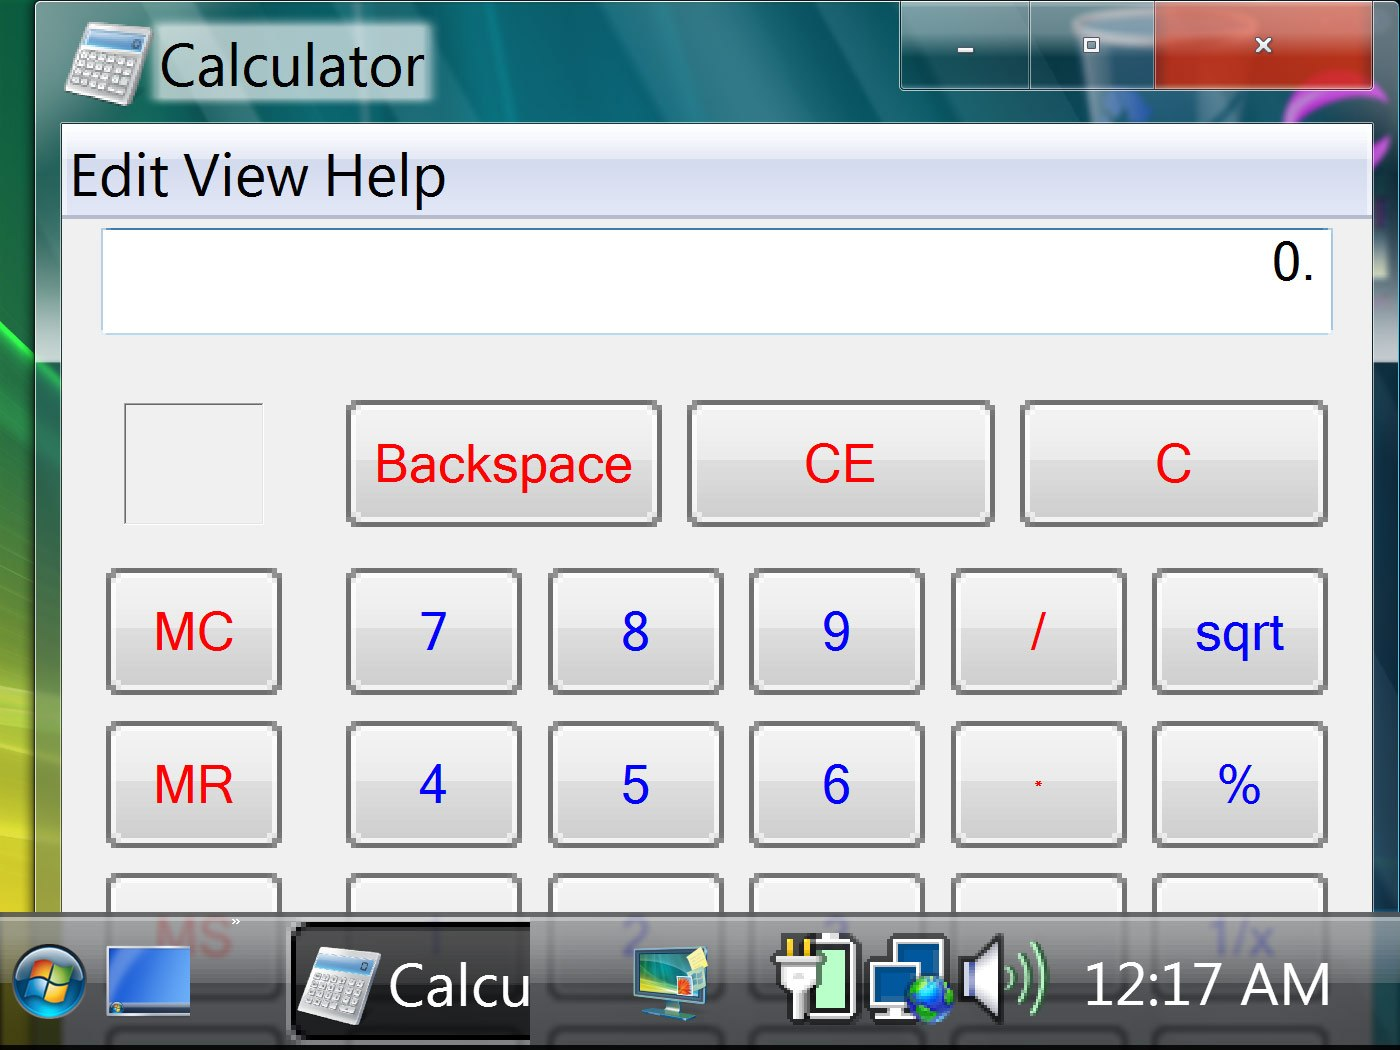
\includegraphics[width=0.8\textwidth]{img/lowres}
\end{frame}

\begin{frame}{Esempio: Finestra non ridimensionabile e alta risoluzione}
\centering
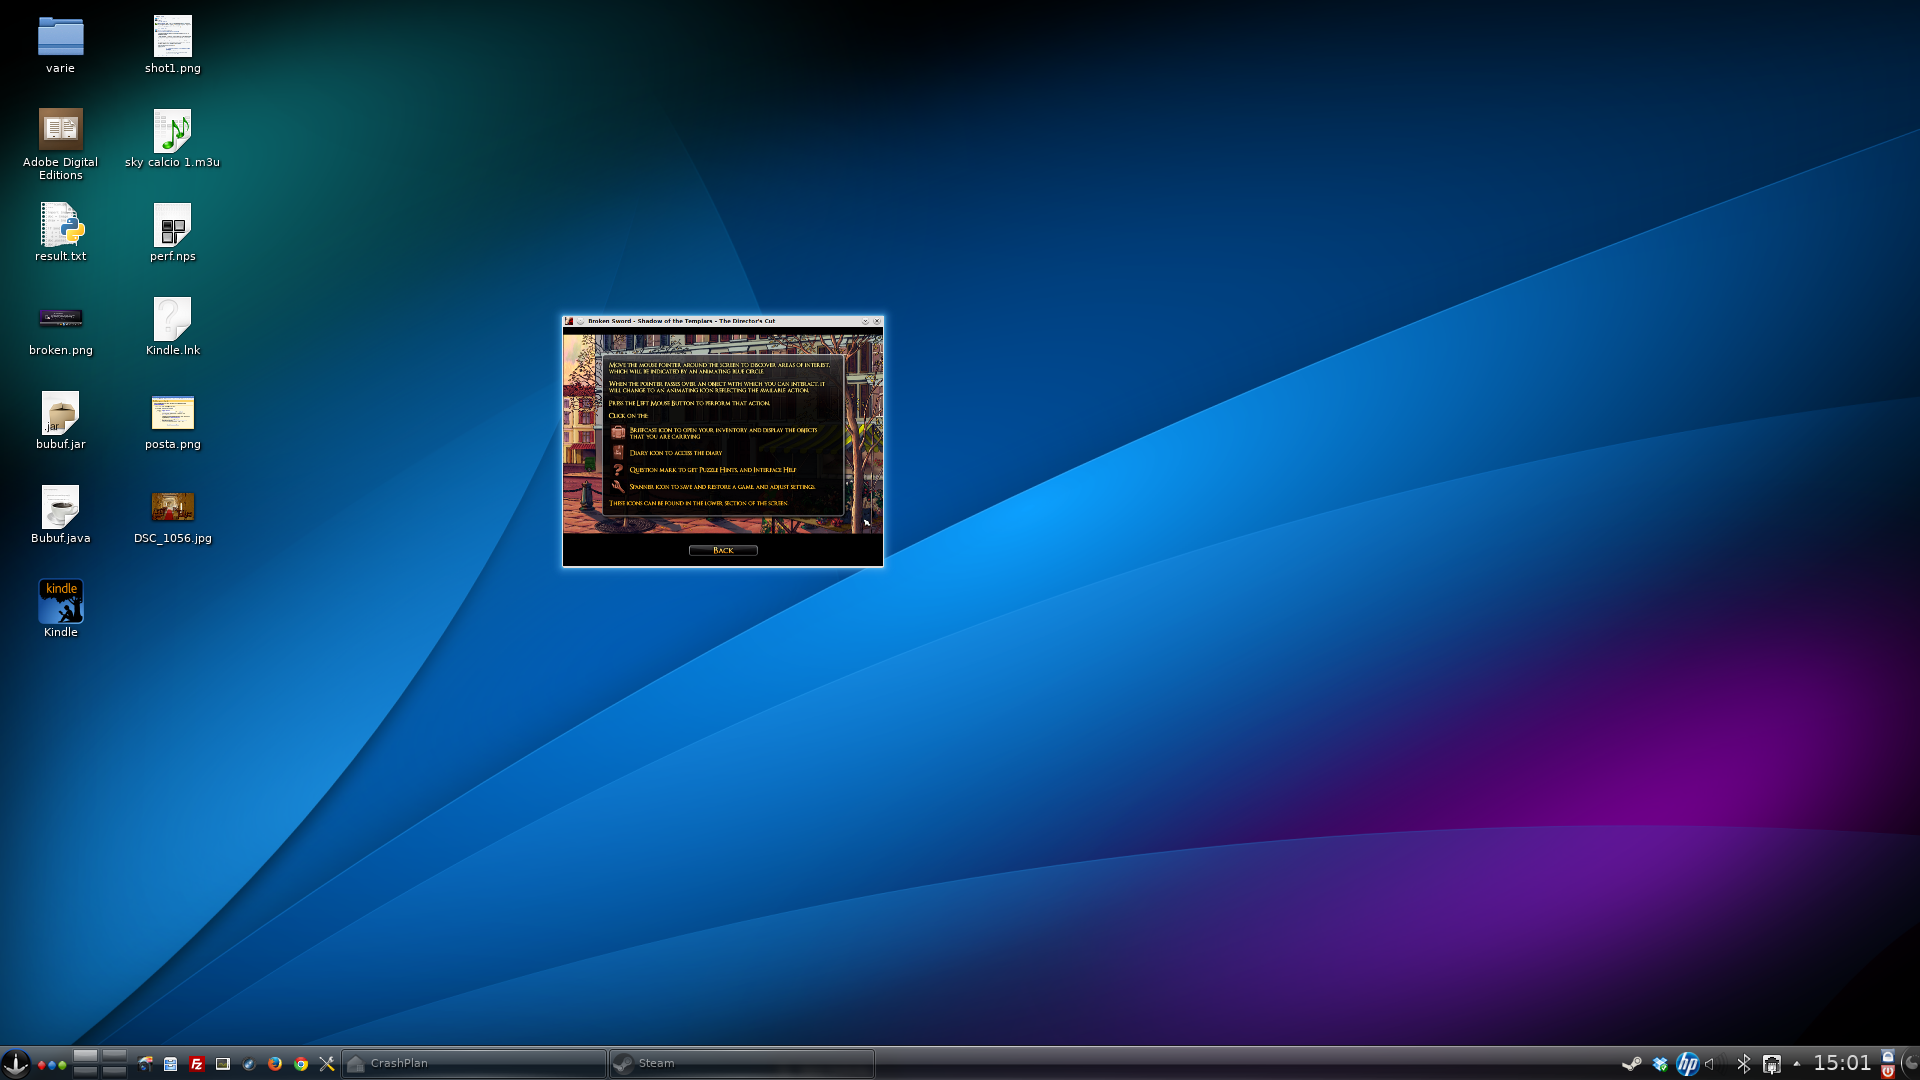
\includegraphics[width=0.8\textwidth]{img/brokensword}
\end{frame}

\begin{frame}{Best-practices per la costruzione di GUI}
\begin{itemize}\itemsep10pt
\item La dimensione di default della finestra va calcolata in base alla dimensione dello schermo.
\item \`{E} opportuno \underline{non} specificare dimensioni assolute in pixel per i componenti della GUI, ma dimensionarli in termini relativi rispetto al container.
\item Anche per i layout è opportuno non utilizzare dimensioni fisse in pixel.
\item I font possono essere allegati all'applicazione
\item La dimensione dei font può essere resa relativa alla dimensione corrente della view.
\item L'ultente deve essere libero di ridimensionare l'interfaccia a piacimento per adattarla alla 
propria configurazione di schermi
\end{itemize}
\end{frame}

\begin{frame}{Supporto multilingua per le UI}
\begin{itemize}
\item Sarebbe opportuno definire la UI una sola volta e cambiare dinamicamente le parti scritte (il testo) a seconda dell'impostazione della lingua di sistema (o della nostra applicazione).
\begin{itemize}
\item In realtà, non solo per la lingua ma anche per il formato dei numeri, la valuta, le convenzioni sulla data,\dots
\end{itemize}
\end{itemize}
\begin{block}{Java Resource Bundles}
Java fornisce una architettura per l'internazionalizzazione, che fa uso di ``\textbf{ResourceBundle}'' e di una serie di file di supporto (properties files).

Per approfondimenti (per implementare il supporto multilingua):
\begin{itemize}
\item \url{https://docs.oracle.com/javase/tutorial/i18n/resbundle/index.html}
\item \url{http://tutorials.jenkov.com/java-internationalization/resourcebundle.html}
\end{itemize}
\end{block}
\end{frame}

\section{Costruzione di un ambiente di sviluppo portabile}

\subsection{Corretta configurazione di un progetto Eclipse, inclusione di librerie}

\begin{frame}{Corretta struttura di un progetto}
	\centering
	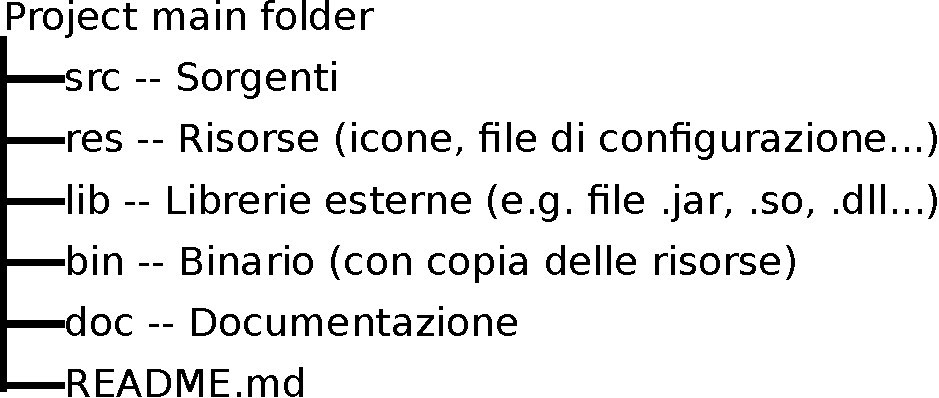
\includegraphics[width=0.99\textwidth]{img/struct}
\end{frame}

\begin{frame}[allowframebreaks]{Corretta struttura di un progetto: Dettagli}
	\begin{block}{\texttt{src}}
		\begin{itemize}
			\item Contiene \textbf{esclusivamente} il codice sorgente dell'applicazione organizzato in package. Non deve contenere altro!
			\item Eventualmente possono esistere più cartelle sorgente.
			\begin{itemize}
				\item Ad esempio perché parte del codice viene generato da un sistema automatico, oppure perché il progetto è sviluppato usando più di un linguaggio.
				\item Nel caso di generatori, è buona norma dividere il codice generato da quello generante, ad esempio creando una cartella \texttt{src-gen}.
				\item Nel caso si utilizzino più linguaggi, è bene distinguerli usando source folder separate, es. \texttt{src-java} e \texttt{src-prolog}.
			\end{itemize} 
			\item In Eclipse è possibile marcare una cartella come ``cartella sorgente'': Proprietà del progetto $\rightarrow$ Java Build Path $\rightarrow$ Source $\rightarrow$ Add Folder $\rightarrow$ Selezione della cartella $\rightarrow$ OK $\rightarrow$ OK
			\begin{itemize}
				\item Tutti i sorgenti di tutte le cartelle sorgente verranno compilati ed inseriti nella cartella di output da Eclipse
			\end{itemize}		
		\end{itemize}
	\end{block}
	\begin{block}{\texttt{res}}
		\begin{itemize}
			\item Contiene le risorse del progetto opportunamente organizzate
			\begin{itemize}
				\item Per risorse si intendono icone, file di testo, video, immagini, modelli 3D e qualunque cosa sia necessaria al corretto funzionamento del programma ma non sia una libreria o un file sorgente.
			\end{itemize}
			\item In Eclipse, per far sì che le risorse vengano inserite nel classpath (da cui sarà più facile caricarle), è necessario rendere \texttt{res} una cartella sorgente con la procedura descritta nella slide precedente.
		\end{itemize}
	\end{block}
	\begin{block}{\texttt{lib}}
		\begin{itemize}
			\item	Contiene tutte le librerie che si sono usate, che siano in file jar o che siano librerie native in formato .so (o .dll)
		\end{itemize}
	\end{block}
	\begin{block}{\texttt{doc}}
		\begin{itemize}
			\item Contiene la documentazione del progetto.
			\item Se si decide di inserire sia documentazione di tipo non rigenerabile (e.g. una relazione in pdf) sia quella di tipo rigenerabile (e.g. la javadoc), è bene tenerle separate.
			\item \textbf{La documentazione rigenerabile non va tracciata col DVCS}
		\end{itemize}
	\end{block}
	\begin{block}{\texttt{bin}}
		\begin{itemize}
			\item Contiene la versione compilata del software.
			\item Contiene una copia delle risorse.
			\item Viene interamente manutenuta dall'IDE.
			\item \textbf{Non va tracciata col DVCS}
		\end{itemize}
	\end{block}
	\begin{block}{\texttt{README.md}}
		\begin{itemize}
			\item File con la descrizione del progetto: autori, breve guida d'uso, link a risorse.
			\begin{itemize}
				\item Bitbucket e GitHub sono in grado di fare il parse del file e di integrarlo nella pagina del progetto, in modo da dargli una descrizione.
			\end{itemize} 
		\end{itemize} 
	\end{block}
\end{frame}

\begin{frame}{Utilizzo di path relativi in Eclipse}
	\begin{itemize}\itemsep20pt
		\item Quando si lavora ad un progetto, \textbf{è bene che tutti i path siano relativi alla radice del progetto stesso}.
		\item In caso contrario:
		\begin{itemize}
			\item Gli altri membri del team dovranno continuamente cambiare le impostazioni per adattarle al loro file system.
			\item Il progetto non sarà sviluppabile su piattaforme diverse.
			\item Si avranno continui merge conflicts se le configurazioni dell'IDE sono in tracking
			\item Le librerie non saranno più accessibili automaticamente
		\end{itemize}
	\end{itemize}
\end{frame}

\begin{frame}[allowframebreaks]{Importazione di librerie Jar in Eclipse}
	\begin{block}{Procedura \textbf{\underline{NON}} corretta}
		Il modo \textbf{\underline{sbagliato}} di cui importare una libreria in Eclipse è: Proprietà del progetto $\rightarrow$ Java Build Path $\rightarrow$ Libraries $\rightarrow$ Add External JARs $\rightarrow$ Selezione dei JAR $\rightarrow$ OK $\rightarrow$ OK
		\begin{itemize}
			\item \`{E} possibile scegliere JAR da qualunque punto del file system.
			\item Vengono generati percorsi assoluti.
		\end{itemize}
	\end{block}
	\begin{block}{Procedura \textbf{\underline{corretta}}}
		Il modo \textbf{\underline{corretto}} di cui importare una libreria in Eclipse è: Proprietà del progetto $\rightarrow$ Java Build Path $\rightarrow$ Libraries $\rightarrow$ Add JARs $\rightarrow$ Selezione dei JAR $\rightarrow$ OK $\rightarrow$ OK
		\begin{itemize}
			\item \`{E} possibile scegliere solo JAR file che esistono in una delle cartelle del progetto (e, se il progetto è ben configurato, sono inserite in \texttt{lib}).
			\item Vengono generati percorsi relativi alla root del progetto.
		\end{itemize}
	\end{block}
\end{frame}

\begin{frame}[allowframebreaks]{Aggiunta di un jar al classpath di un progetto Eclipse}
	\begin{block}{}
		Progetto $\rightarrow$ Properties $\rightarrow$ Java build path $\rightarrow$ Libraries 
$\rightarrow$ Add Jar
	\end{block}
	\begin{center}
		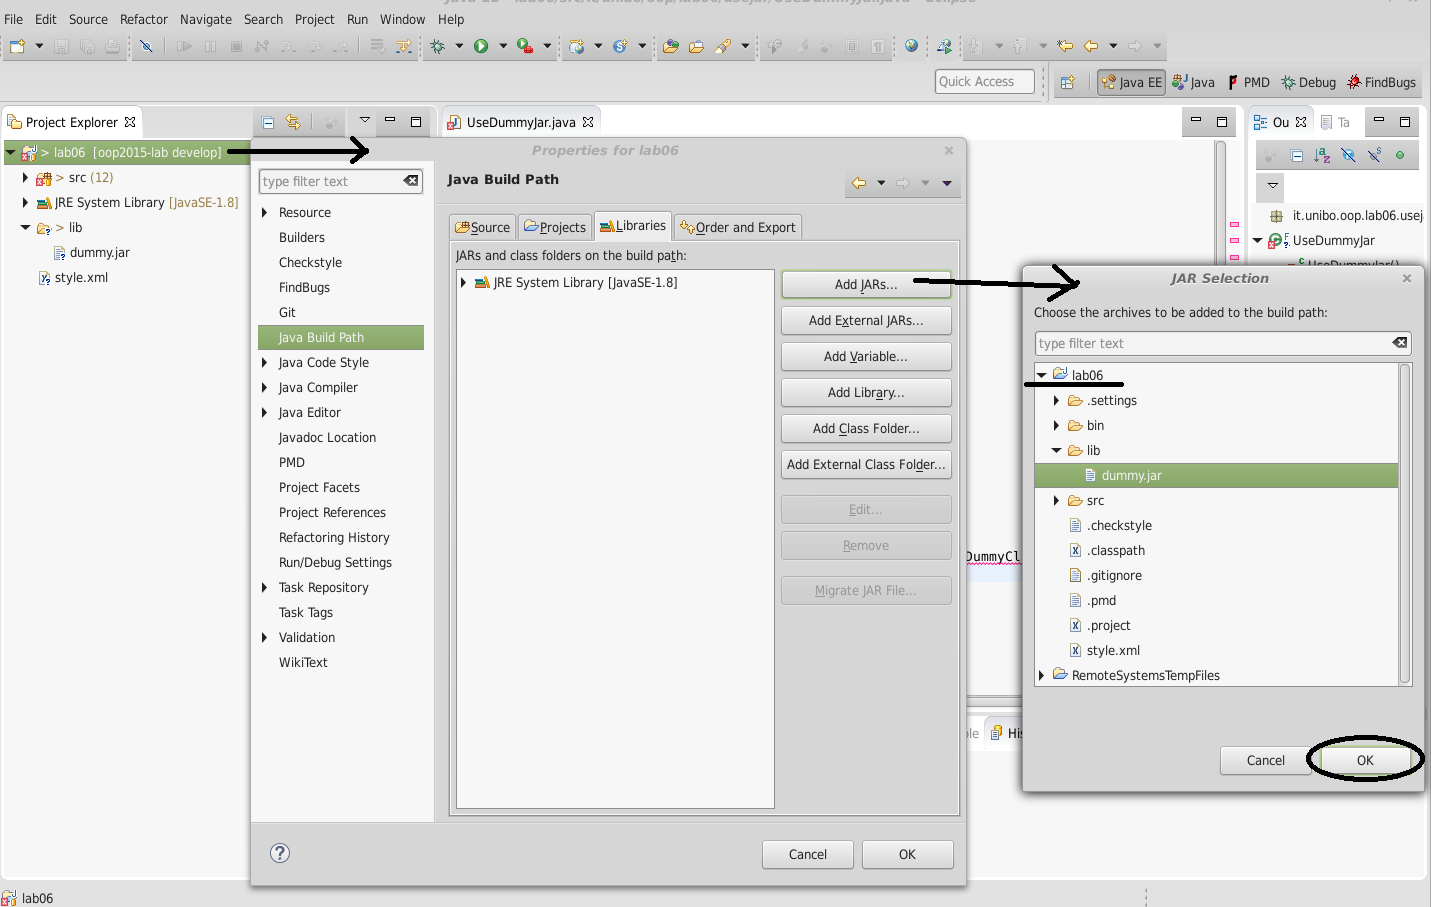
\includegraphics[width=0.82\textwidth]{img/addjar-1} \\
		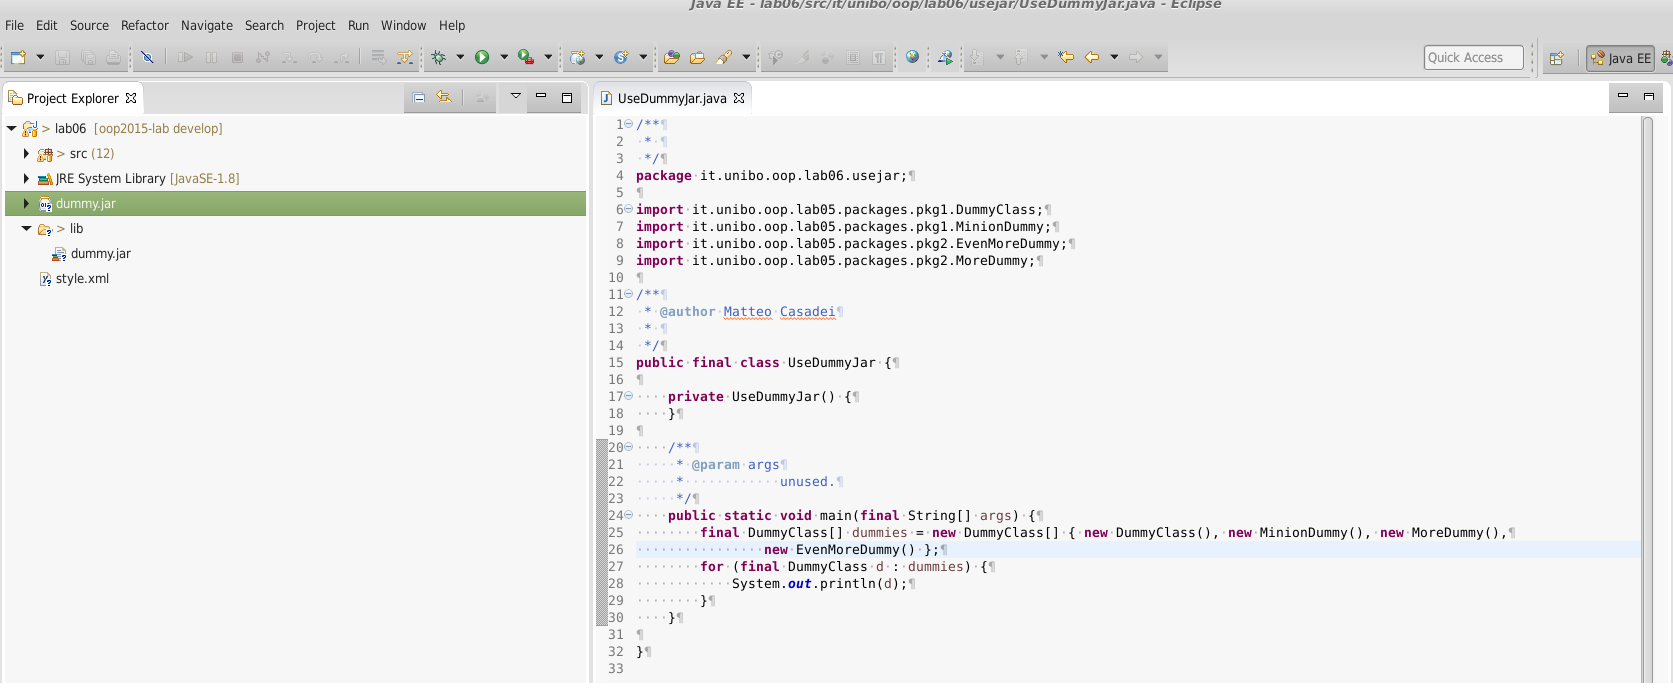
\includegraphics[width=0.99\textwidth]{img/addjar-2} \\
		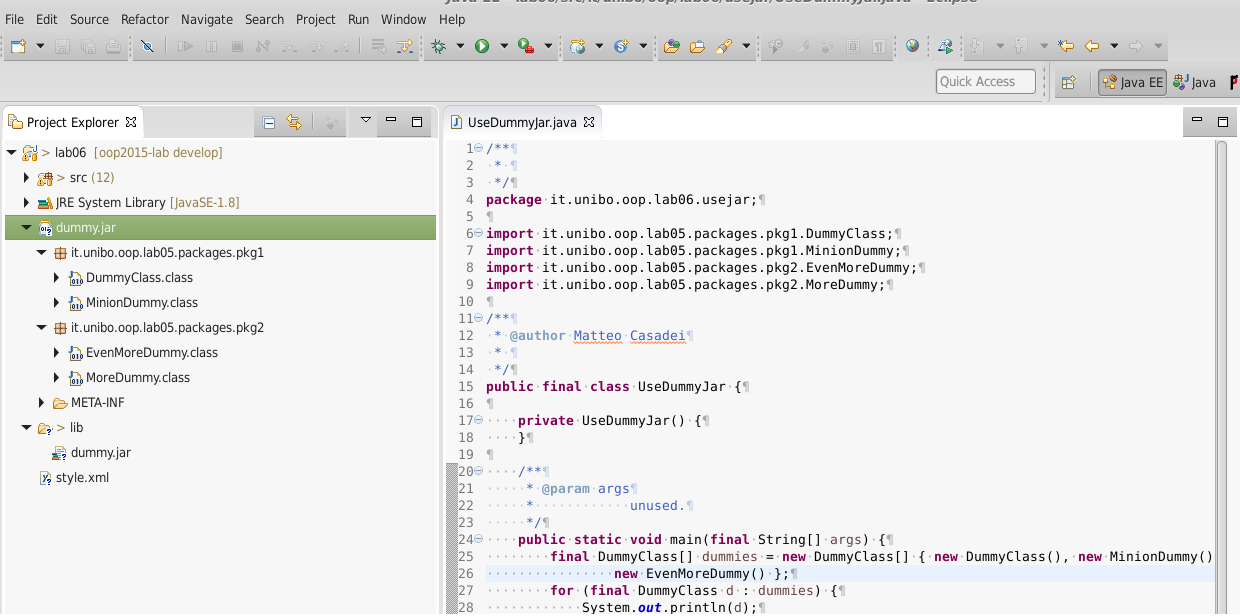
\includegraphics[width=0.99\textwidth]{img/addjar-3} \\
	\end{center}
\end{frame}

\subsection{Font ed encoding}

\begin{frame}{Font ed encoding}
	Le più note piattaforme utilizzano di default encoding diversi:
	\begin{itemize}
		\item \textbf{UTF-8} --- default su Linux, può essere considerato lo standard de-facto.
		\item \textbf{MacRoman} --- default su MacOS, raramente causa artefatti se riconvertito ad altri formati.
		\item \textbf{ISO-8859-1} --- default su Windows, può causare artefatti su quasi tutti i caratteri non ASCII se convertito a UTF-8.
	\end{itemize}
	\begin{block}{Encoding per il codice sorgente}
		Solitamente, il codice sorgente si sviluppa utilizzando la codifica UTF-8
		\begin{itemize}
			\item Essenziale se si utilizzano caratteri non inclusi nella tabella ASCII (caratteri accentati, ad esempio).
		\end{itemize}
	\end{block}
\end{frame}

\begin{frame}[allowframebreaks]{Carattere di new line}
	Unix e Windows differiscono anche per il carattere di newline
	\begin{itemize}
		\item \texttt{\textbackslash{}n} --- Su Linux e MacOS X (e su tutti i sistemi non Windows).
		\item \texttt{\textbackslash{}r} --- Su MacOS 9 e precedenti
		\item \texttt{\textbackslash{}r\textbackslash{}n} --- Windows
	\end{itemize}
	\begin{block}{Pillola di storia}
		\begin{itemize}
			\item Il ``carriage report'' è un'eredità dovuta alla compatibilità con MS-DOS
			\item Che a sua ha ereditato la cosa dalla compatibilità con CP/M-80
			\item A quel tempo, le stampanti erano macchine da scrivere elettromeccaniche
			\item \texttt{\textbackslash{}r} riportava il rullo con la carta al margine sinistro
			\item Anche se queste stampanti non sono più in uso, alcuni produttori (come HP) mantengono la compatibilità su alcuni prodotti
			\item Ad oggi, si usa \texttt{\textbackslash{}r} solo per realizzare animazioni su terminale (far sì che la nuova linea cancelli la precedente)
		\end{itemize}
	\end{block}
	\begin{block}{Standardizzazione}
		\begin{itemize}
			\item Entrambi i sistemi ``digeriscono'' entrambi i newline
			\item Ma se due membri del team usano impostazioni diverse, il DVCS considererà ogni file modificato come integralmente cambiato ad ogni salvataggio 
			\begin{itemize}
				\item Diff incomprensibili
				\item Storia del progetto compromessa
				\item Difficoltà di produrre patch e ripristinare il lavoro precedente
			\end{itemize}
			\item Facciamo una scelta, e utilizziamo un solo formato
			\item La nostra scelta sarà \texttt{\textbackslash{}n} (Unix newline)
		\end{itemize}
	\end{block}
\end{frame}

\begin{frame}{Configurazione di encoding e newline in Eclipse}
	\begin{itemize}
		\item Selezione del progetto $\rightarrow$ Click destro $\rightarrow$ Preferences $\rightarrow$ Resource
		\item Text file encoding $\rightarrow$ Other $\rightarrow$ UTF-8
		\item New text file line delimiter $\rightarrow$ Other $\rightarrow$ Unix
		\item Apply $\rightarrow$ OK
	\end{itemize}
	\begin{center}
	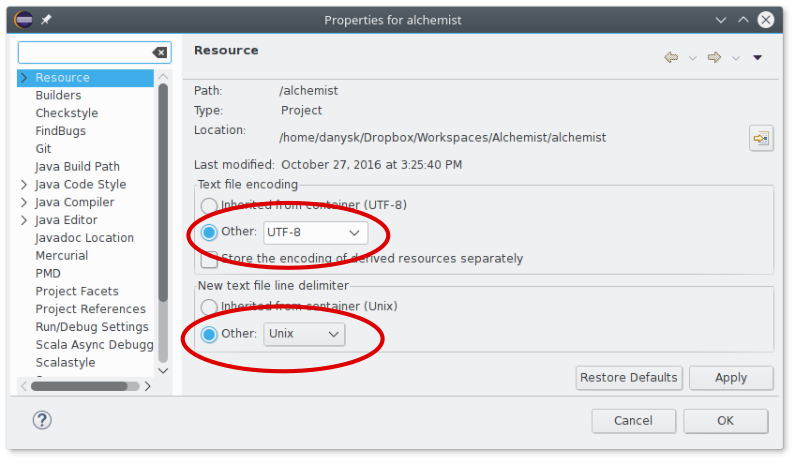
\includegraphics[width=0.8\textwidth]{img/eclipse-encoding}
	\end{center}
\end{frame}

\subsection{Caricamento di risorse dal classpath}

\begin{frame}{Risorse caricate dal classpath}
	\begin{itemize}
		\item Abbiamo visto finora il classpath come l'insieme dei percorsi dove la virtual machine va a cercare le classi da caricare
		\item Esso include anche i contenuti di tutte le cartelle sorgente, che Eclipse copierà dentro la cartella \texttt{bin}, e che includerà nel JAR eseguibile assieme ai file compilati
		\item Come possiamo accedere a queste risorse in modo trasparente?
		\begin{itemize}
			\item Ossia caricarle sia che si trovino sul file system, sia che si trovino nel JAR eseguibile, sia che vengano incluse in un JAR di risorse separato.
		\end{itemize} 
	\end{itemize}
	\begin{block}{\texttt{Class.getResource()}}
		\begin{itemize}
			\item Java fornisce un'utilità per caricare risorse dal \textbf{classpath}
			\item Come abbiamo visto usando l'opzione \texttt{-cp} di \texttt{java} e \texttt{javac}, il classpath può contenere indifferentemente dei path o dei JAR (o anche degli zip)
		\end{itemize}
		\end{block}
\end{frame}

\begin{frame}[fragile]{Risorse caricate dal classpath -- Esempi}

\begin{block}{Caricamento di File}
\begin{lstlisting}
final InputStream in = LoadImage.class.getResourceAsStream("/settings/settings");
final BufferedReader br = new BufferedReader(new InputStreamReader(in));
final String line = br.readLine();
in.close();
\end{lstlisting}
\end{block}

\begin{block}{Caricamento di Immagini}
\begin{lstlisting}
final URL imgURL = LoadImage.class.getResource("/images/gandalf.jpg");
final ImageIcon icon = new ImageIcon(imgURL);
final JLabel lab1 = new JLabel(icon);
\end{lstlisting}
\end{block}
\end{frame}

\subsection{Installazione delle impostazioni per-utente}

\begin{frame}{Installazione delle impostazioni}
\begin{block}{Motivazione}
Spesso un software ha necessità di caricare al primo avvio delle impostazioni di default, quindi lasciare l'utente libero di modificarle e, se avviato successivamente caricare quelle scelte dall'utente. In caso di sistema multiutente, le impostazioni saranno diverse per ciascuno.
\end{block}

\begin{block}{Strategia}
\begin{itemize}
\item Si sceglie una cartella nella home folder dell'utente dove salvare le impostazioni. 
\begin{itemize}
\item È norma consolidata creare una cartella \texttt{.nomeprogramma}.
\end{itemize}

\item Al primo avvio, si verifica se tale cartella esista e se contenga i file di configurazione previsti.
\begin{itemize}
\item Se non è presente, o se non sono presenti e leggibili alcuni i file, si procede a caricare 
nella cartella di destinazione i file di default dal jar usando \texttt{getResource()}.
\end{itemize}
\end{itemize}
\end{block}
\end{frame}

\section{Ricerca/Utilizzo di librerie}
\begin{frame}{Uso di Librerie}
	\begin{itemize}\itemsep15pt
		\item Durante lo sviluppo di un software, spesso emerge la necessità di realizzare componenti a supporto della propria applicazione, utili per incapsulare un determinato comportamento/funzionalità ma non cruciali per la logica applicativa.
		\item Nella maggior parte dei casi una tale libreria/componente è già stato sviluppato da qualcun altro!
		\item Risulta opportuno avvalersi di librerie già disponibili e testate\dots
		\begin{itemize}
			\item \dots dopo aver letto attentamente la documentazione e averne compreso a fondo il comportamento!
		\end{itemize}
	\end{itemize}
\end{frame}

\begin{frame}{Librerie particolarmente utili}
	\begin{itemize}\itemsep15pt
		\item \textbf{Google Guava} (\url{https://github.com/google/guava})
		\begin{itemize}
			\item Il progetto Guava di Google raccoglie diverse librerie core sviluppate da Google che possono essere utilizzate per lo sviluppo di applicazioni.
			\item Ad esempio, sono disponibili librerie per Collections Management, Concurrency, I/O, String Processing,\dots
		\end{itemize}
		\item \textbf{Apache Commons} (\url{https://commons.apache.org})
		\begin{itemize}
			\item Estensioni al linguaggio (Commons Lang3)
			\item Libreria matematica estesa (Commons Math3)
			\item Accesso semplificato all'I/O (Commons IO)
			\item Costruzione semi automatica di una command line (Commons CLI)
			\item Encoding e crittazione (Commons Codec), compressione (Commons Compress)
		\end{itemize}
		\item \textbf{Static Logger Facade for Java (SLF4J)} (\url{http://www.slf4j.org})
		\begin{itemize}
			\item Backend-independent logging (addio \texttt{println})
		\end{itemize}
	\end{itemize}
\end{frame}

\begin{frame}{Top 20 Java Library}
	\begin{center}
		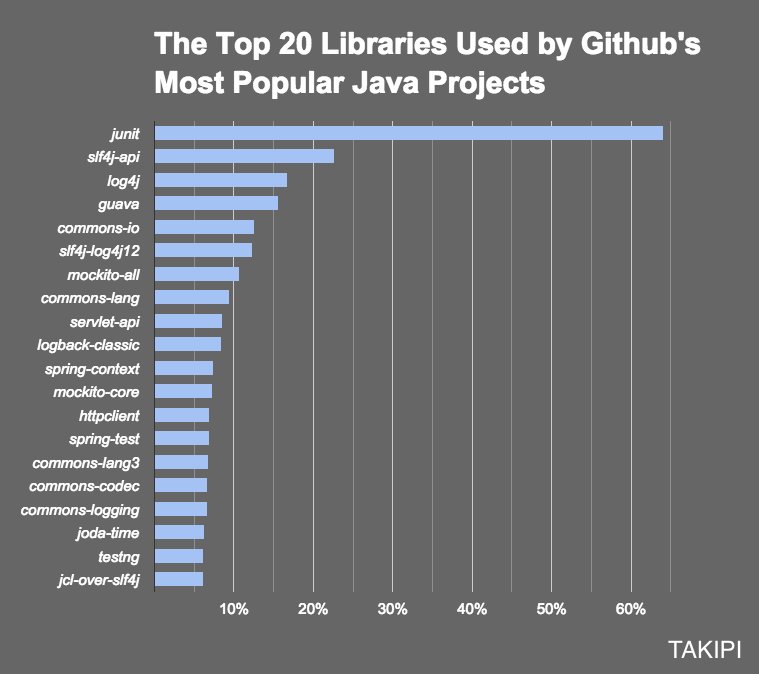
\includegraphics[width=0.6\textwidth]{img/top-20-java-libraries}
	\end{center}
	{\scriptsize \url{blog.takipi.com/we-analyzed-60678-libraries-on-github-here-are-the-top-100}}
\end{frame}

\begin{frame}{Awesome Java}
	Esiste una lista, costantemente manutenuta, che elenca le più comuni, diffuse e stabili librerie per una pletora di usi:
	\begin{center}
		\url{https://bit.ly/awesome-java}
	\end{center}
	\begin{center}
		\begin{LARGE}\textbf{U-SA-TE-LE}\end{LARGE}
	\end{center}
	\begin{center}
		\textbf{Usare librerie e non reinventare la ruota è \alert{IMPORTANTE} e valutato 
positivamente.}
	\end{center}
		Attenzione però a scegliere le librerie dopo aver fatto il \textbf{modello del dominio} 
dell'applicazione: \textbf{PRIMA} si studia il problema, \textbf{DOPO} si implementa una soluzione: 
siete aspiranti ingegneri, cercate di lavorare sempre top-down quando possibile, non partite dalla 
libreria per costruirci sopra un software, ma partite dai requisiti e - se utile - sfruttate le 
librerie per soddisfarli.
\end{frame}

\begin{frame}{The Maven Central Repository}
\begin{itemize}\itemsep10pt
\item Costituisce la più ampia collezione di librerie e componenti Java open-source.
\begin{itemize}
\item È il repository di default per Apache Maven (noto tool per il project management).
\end{itemize}
\item Rappresenta uno dei modi più rapidi per accedere a librerie sviluppate da altri sviluppatori e distribuire le proprie.
\item Consente di ricercare e scaricare pressoché qualunque libreria a supporto utile nelle proprie applicazioni open-source.

\item \url{https://search.maven.org/}
\end{itemize}
\end{frame}

\section{Qualità  del codice}
\subsection{Strumenti per il controllo di qualità}
\begin{frame}{Analisi di qualità  del codice sorgente}
	\begin{block}{Definizione}
		Software in grado di analizzare il codice sorgente per individuare:
		\begin{itemize}
			\item Potenziali bug, magari dovuti a distrazione
			\item Possibili miglioramenti, ottimizzazioni o pratiche difformi da quelle consigliate
			\item Codice duplicato, segnale di una progettazione discutibile
			\item Stile non conforme
		\end{itemize}
	\end{block}
	\begin{block}{Uso}
		L'analisi automatica del proprio codice garantisce sempre un elevata qualità  del codice, aiuta ad apprendere il modo corretto di scrivere, riduce il costo di manutenzione e garantisce uniformità  fra le parti sviluppate da persone diverse.
	\end{block}
\end{frame}

\begin{frame}[allowframebreaks]{Code checking}
	I software che vedremo sono eseguibili in due modalità \footnote{In realtà  cominciano a prender piede anche servizi web come Codacy, ma non li tratteremo in questo corso...}:
	\begin{itemize}
		\item Stand-alone: il software viene eseguito e genera un report
		\item Come plug-in: il software viene integrato con l'IDE (nel nostro caso Eclipse), e segnala i problemi sotto forma di warning
	\end{itemize}
	Noi ci concentreremo nell'imparare la seconda modalità .
\end{frame}

\begin{frame}[allowframebreaks]{Code checkers in Eclipse}
	\begin{block}{Installazione}
		Per l'installazione, si seguano le istruzioni fornite sulla pagina dei installazione del software del corso.
	\end{block}
	\begin{block}{Configurazione globale}
	La configurazione globale viene applicata a \textbf{tutti} i progetti del workspace, a meno che non sia sovrascritta localmente (non sempre è possibile).
		\begin{itemize}
			\item Veloce da configurare: si configura una volta, e i settaggi sono applicati su tutti i progetti
			\item Poco portabile: se inviamo il progetto ad un collaboratore, questi settaggi \textbf{non} saranno inviati: c'è il rischio di inconsistenze
			\item Ottimo da usare quando si hanno molti progetti nel workspace con la stessa configurazione, e si sviluppa da soli.
		\end{itemize}
	\end{block}
	\begin{block}{Configurazione locale}
	La configurazione locale va messa a punto singolarmente per ciascun progetto. Bisogna verificare che quella globale non la stia sovrascrivendo.
		\begin{itemize}
			\item Alta flessibilità: si possono specificare regole diverse per progetti diversi
			\item Alta portabilità: se si invia il progetto ad un collaboratore, queste impostazioni
vengono mantenute
			\item Ottimo da usare quando si hanno pochi progetti, o ai progetti serve una configurazione diversa, oppure quando si lavora in modo collaborativo
		\end{itemize}
	\end{block}
	\begin{center}
		Noi faremo uso della configurazione \textbf{locale} \\
		\textbf{Voi farete} uso della configurazione locale nell'\textbf{elaborato finale}
	\end{center}
\end{frame}

\fr{SpotBugs (ex FindBugs)} {
  \bl{Cos'è} {
      SpotBugs scansiona il bytecode generato dal compilatore, e dalla sua analisi cerca di scoprire potenziali bug nel sorgente, ad esempio:
      \iz {
        \item Uguaglianza esatta fra \texttt{float} o \texttt{double}
        \item Utilizzo di \texttt{==} invece di \texttt{equals()}
        \item Mancata annotazione di annotazioni usate a runtime via reflection
        \item Uso errato di meccanismi di sincronizzazione
        \item Vulnerabilità  di sicurezza
        \item Tanti altri! Si veda: \url{http://findbugs.sourceforge.net/bugDescriptions.html}
      }
  }
}

\fr{SpotBugs --- Configurazione globale} {
	\centering
	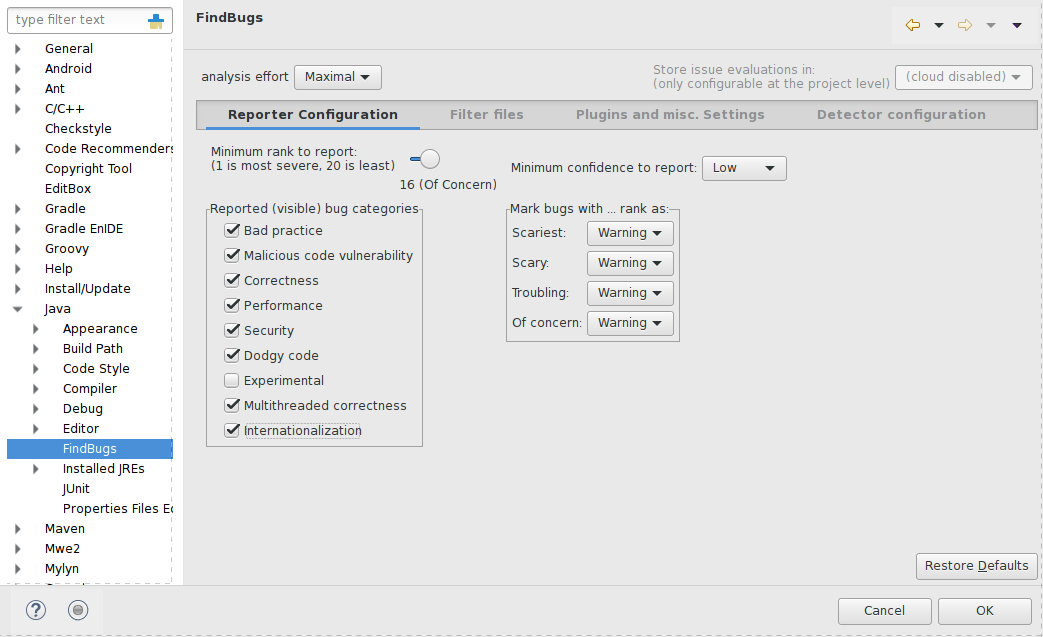
\includegraphics[width=0.99\textwidth]{img/findbugsconf}
}

\fr{SpotBugs --- Configurazione del progetto} {
  In SpotBugs, la configurazione locale \textbf{è più prioritaria} di quella globale.
  \centering
  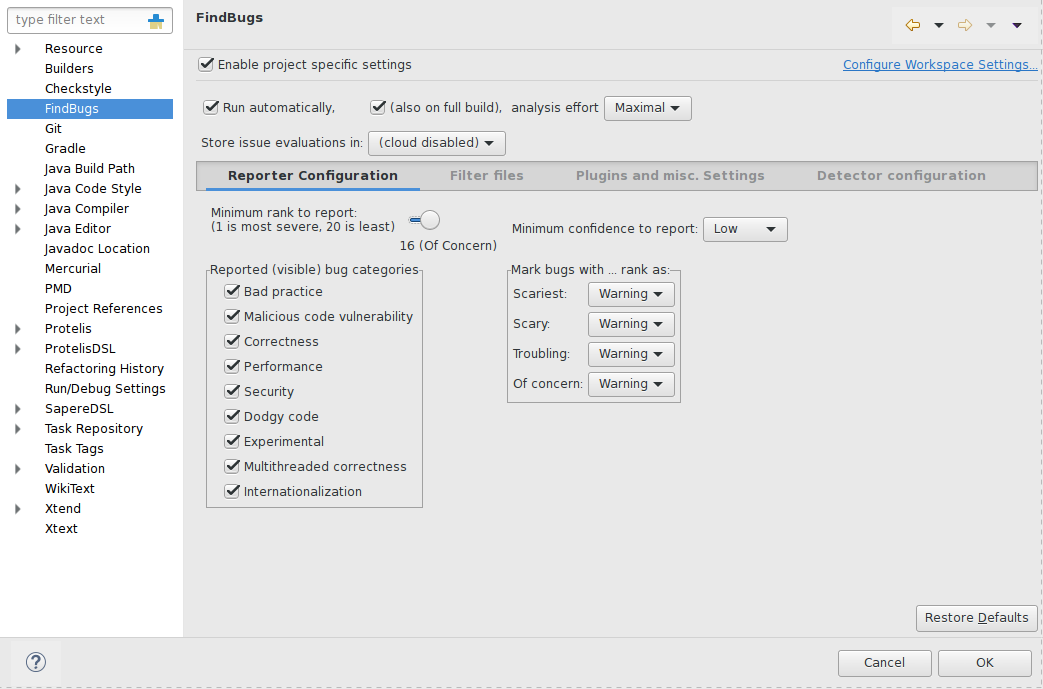
\includegraphics[width=0.9\textwidth]{img/findbugsproj}
}

\fr{PMD e CPD} {
	\bl{Cos'è} {
		PMD si occupa di trovare imperfezioni nel codice:
		\iz {
			\item Campi pubblici, protetti o default
			\item Mancato uso di final
			\item Singular fields
			\item Usa CPD per verificare se vi siano blocchi di codice copincollati
			\item Tanti altri! Si veda: \url{http://pmd.sourceforge.net/pmd-4.3.0/rules/index.html}
		}
	}
}

\fr{PMD --- Configurazione globale} {
	La configurazione di default di PMD contiene regole con limiti arbitrari, regole che hanno senso solo in particolari environment (e.g. J2EE) e regole controverse. È meglio rimuovere tali regole!
	\iz{
		\item Dalle proprietà  di Eclipse, si allarghi il sotto menu PMD
		\item Si vada su Rule Configuration
		\item Si selezionino tutte le regole (click su una, poi ctrl+A)
		\item Si eliminino tutte le regole
		\item Si usi il tasto import
		\item Si importino (meglio per copia) le regole da un file XML
		\item Vi forniremo noi un buon file di regole!
	}
}

\fr{PMD --- Configurazione globale} {
	\centering
	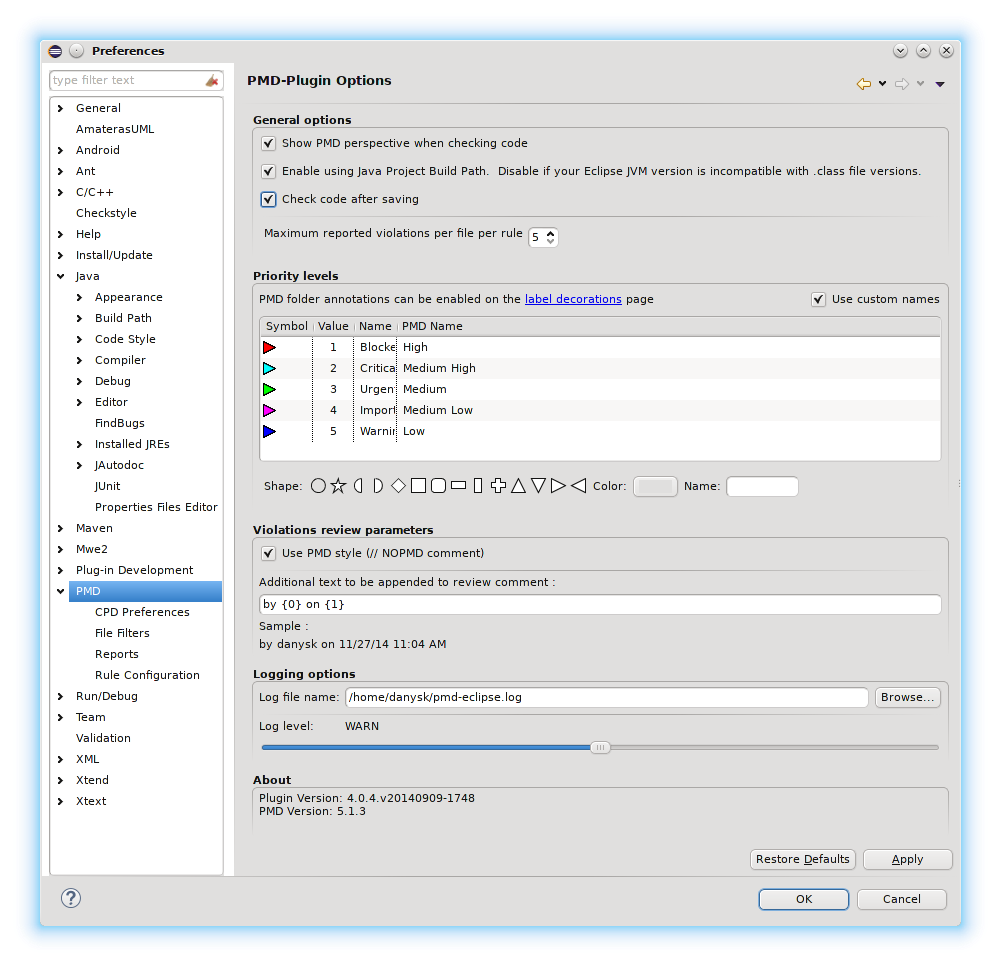
\includegraphics[width=0.75\textwidth]{img/pmdconf}
}

\fr{PMD --- Configurazione globale} {
  In PMD, la configurazione globale \textbf{sovrascrive} quella locale: \textbf{disattivate} ``Use 
global rule management''
  \centering
  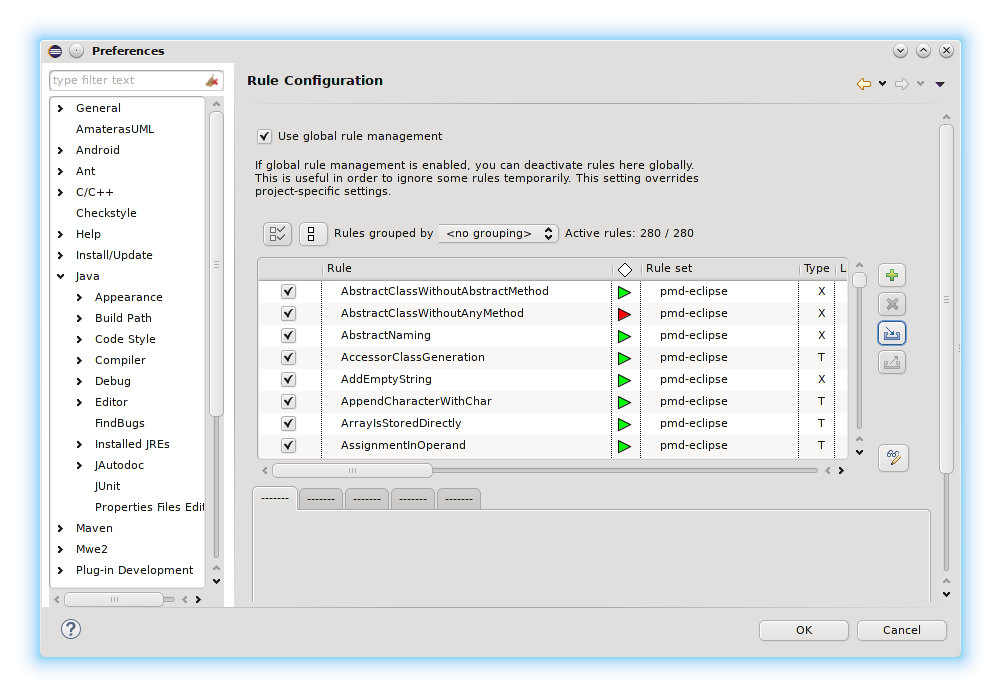
\includegraphics[width=0.9\textwidth]{img/pmdconf1}
}

\fr{PMD --- Configurazione globale} {
	\centering
	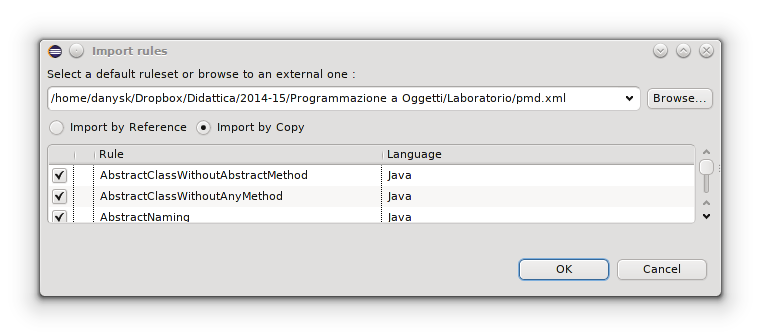
\includegraphics[width=0.99\textwidth]{img/pmdimport}
}

\fr{PMD --- Configurazione del progetto} {
    \centering\textcolor{red}{ATTENZIONE}
    \begin{itemize}
        \item Prima di attivare la configurazione locale, \textbf{assicurarsi} 
che il file pmd.xml sia stato copiato all'interno della cartella del progetto!
        \item Non usare ``Browse...'', o il plugin genererà un percorso 
assoluto!
    \end{itemize}
	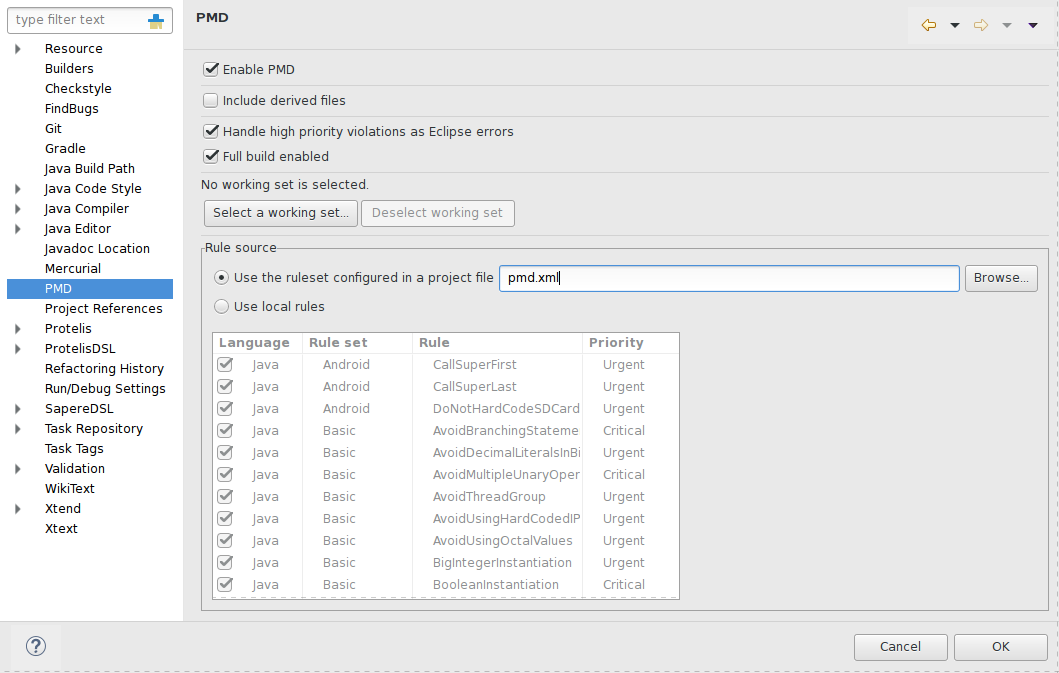
\includegraphics[width=0.8\textwidth]{img/pmdproj}
}

\fr{Checkstyle} {
	\bl{Cos'è} {
		Checkstyle si occupa di trovare errori di stile:
		\iz {
			\item Mancanza di commento Javadoc
			\item Spaziature non corrette
			\item Parentesi assenti
			\item Magic numbers
			\item Altro: \url{http://checkstyle.sourceforge.net/checks.html}
		}
	}
}

\fr{Checkstyle --- Configurazione} {
	La configurazione di default di Checkstyle è eccessivamente pedante. Vi forniremo noi un file di configurazione idoneo:
	\en{
		\item Dalle proprietà  di progetto, si clicki sul menu Checkstyle
		\item Si selezioni ``Local Check Configurations''
		\item Si scelga ``New''
		\item Si scelga ``Project Relative Configuration'' (mai usare path assoluti!)
		\item Utilizzando ``Browse...'' si punti al file di configurazione, che deve esser copiato nel progetto
		\item Si dia un nome e si prema ``OK''
		\item Si vada su ``Main''
		\item Si selezioni dal menu la nuova Check configuration
		\item Si attivi ``Checkstyle active for this project'' e ``Use simple configuration''
		\item ``OK''
	}
	\footnotesize
	Nota: la configurazione globale è molto simile, si ripetano gli step andando dal menu  Windows $\rightarrow$ Preferences $\rightarrow$ Java $\rightarrow$ Code style $\rightarrow$ Formatter 
}

\fr{Checkstyle --- Configurazione per-progetto} {
	\centering
	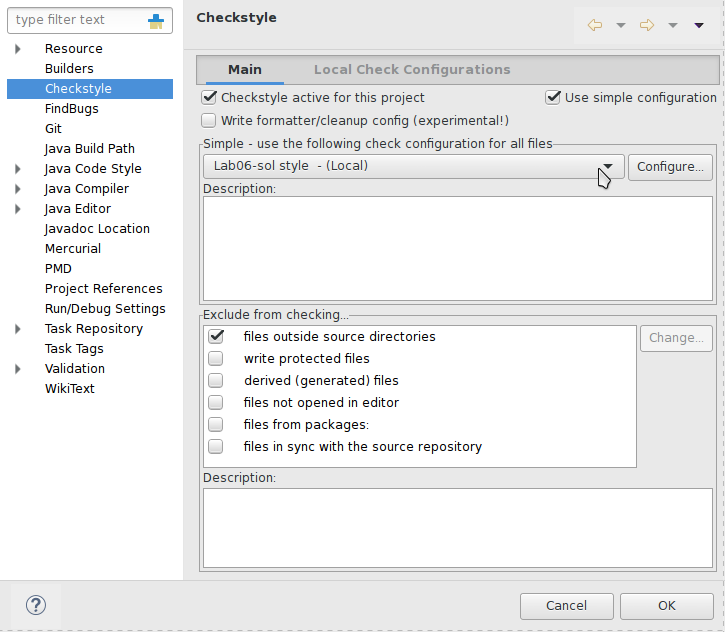
\includegraphics[width=0.7\textwidth]{img/checkstyle}
}

\subsection{Coding style: configurazione IDE Eclipse}
\fr{Configurare l'IDE per una corretta formattazione del codice} {
	Checkstyle è in grado di supportarci nel verificare l'utilizzo di un corretto stile di codifica. Adattando le ``Java Code Convention'':
	\iz{
		\item 4 spazi per l'indentazione
		\begin{itemize}
			\item Nell'originale è consentito scegliere fra fra i due ed i quattro
		\end{itemize}
		\item Nessun carattere tab
		\begin{itemize}
			\item Nell'originale è consentito usarli
			\item Ma noi vogliamo indentazione consistente, quindi o spazi, oppure tab
			\item Essendo in JCC un tab equivalente ad 8 spazi, diventa troppo largo per una buona indentazione 
		\end{itemize}
		\item Linee lunghe al massimo 120 o 130 caratteri
		\begin{itemize}
			\item Nell'originale sono 80 per motivi storici (le schede perforate IBM avevano 80 colonne)
			\item Noi abbiamo i monitor, e anche i nostri colleghi
		\end{itemize}

	}
	\begin{block}{}
		Ora, però, dobbiamo configurare l'editor perché ci supporti nella scrittura di codice con lo stile corretto: come fare?
	\end{block}
}

\begin{frame}[allowframebreaks]{Configurazione del formattatore di Eclipse}
	\begin{center}
		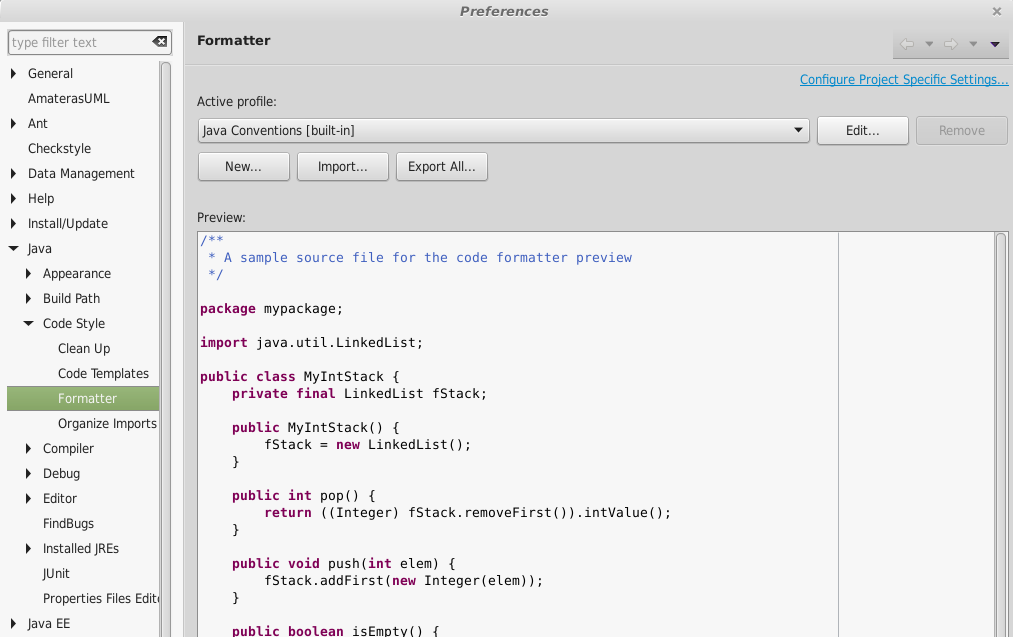
\includegraphics[width=.95\textwidth]{img/ideconf-1} 
	\end{center}
	\begin{center}
		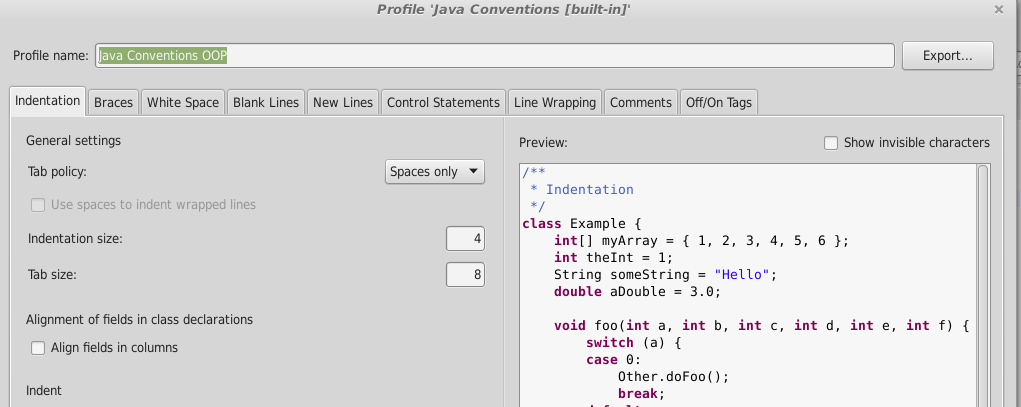
\includegraphics[width=\textwidth]{img/ideconf-2}
	\end{center}
	\begin{center}
		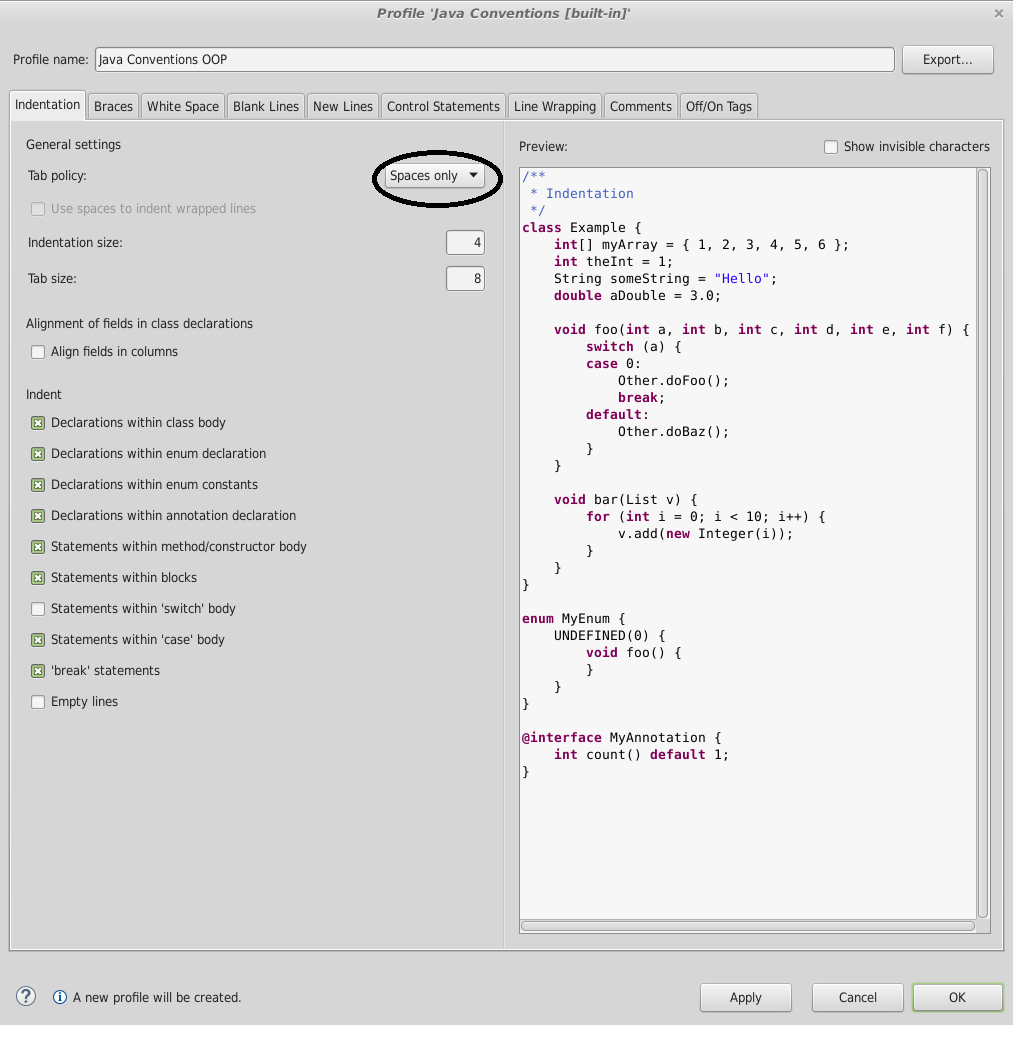
\includegraphics[width=\textwidth]{img/ideconf-3}
	\end{center}
	\begin{center}
		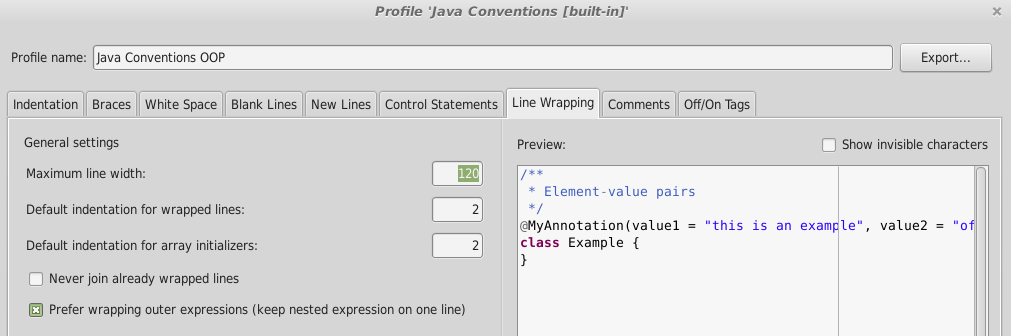
\includegraphics[width=\textwidth]{img/ideconf-4}
	\end{center}
\end{frame}

\section{Ispezione e Profiling con VisualVM}

\begin{frame}{Profiling di applicazioni Java}
\begin{itemize}\itemsep10pt
\item Quando si sviluppa un'applicazione complessa, soprattutto se basata su meccanismi di concorrenza, è opportuno analizzarne il comportamento e monitorarne le performance.
\begin{itemize}
\item Spesso il monitoraggio delle performance è essenziale per identificare eventuali problematiche o capire l'origine di problemi che possono essere sorti.
\end{itemize}
\item Tra gli strumenti che possono essere utilizzati per monitorare l'esecuzione di applicazioni che sono eseguite sulla JVM, due sono distribuiti unitamente al Java Development Kit (JDK).
\begin{itemize}
\item \textbf{JConsole}, lo storico (e scarno) tool per il profiling di applicazioni Java.
\item \textbf{JVisualVM}, il più recente ed evoluto tool utilizzabile per monitorare l'evoluzione e le performance di applicazioni in esecuzione sulla JVM.
\end{itemize}
\end{itemize}
\end{frame}

\begin{frame}{VisualVM}
\begin{itemize}\itemsep10pt
\item Si tratta di un profiler per applicazioni Java che consente di misurarne ed analizzarne le performance.
\item Interagisce con la JVM per fornire informazioni circa le performance e il consumo di risorse di applicazioni in esecuzione.
\item Distribuito internamente al JDK dalla versione 5.0
\item Consente di monitorare:
\begin{itemize}
\item la percentuale di CPU utilizzata da singoli metodi, thread, \dots
\item per quanto tempo un thread si trova nello stato di running oppure in stato di blocco o di idle.
\item \dots
\end{itemize}
\item Richiamabile attraverso il comando \texttt{jvisualvm} o \texttt{visualvm} (dipendentemente dalla distribuzione Java).
\end{itemize}
\end{frame}

\begin{frame}{VisualVM - Overview}
\centering
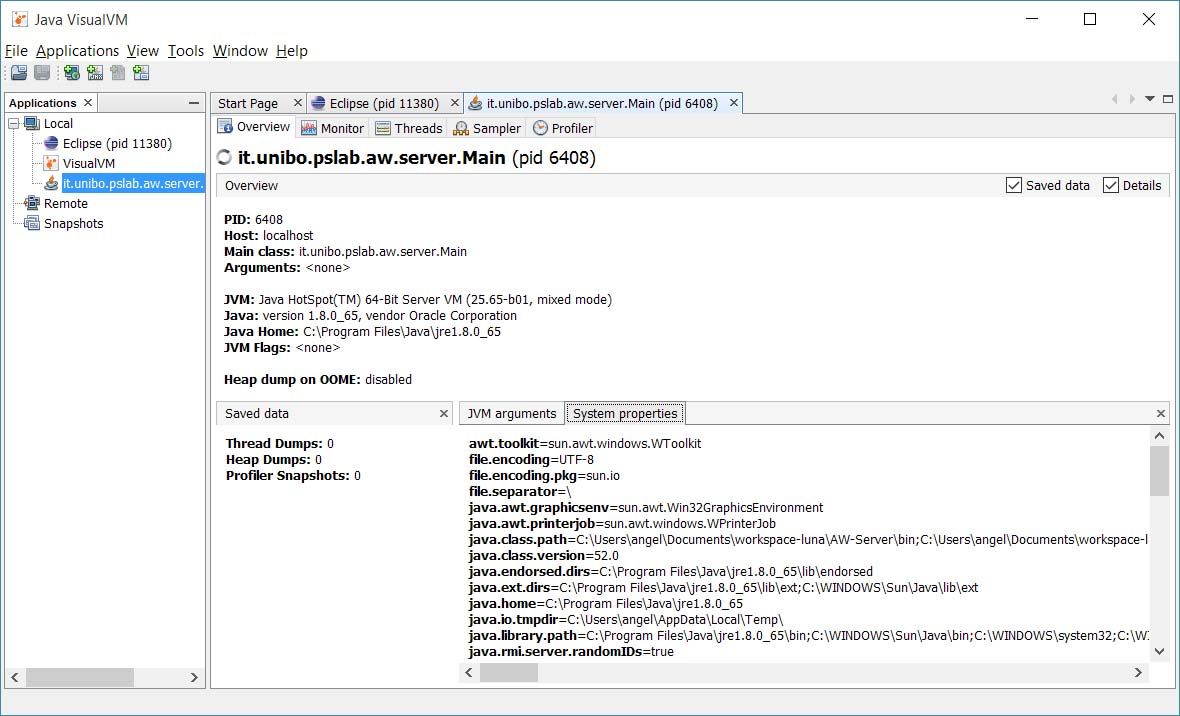
\includegraphics[width=0.99\textwidth]{img/jvisualvm-0}
\end{frame}

\begin{frame}{VisualVM - Monitor}
\centering
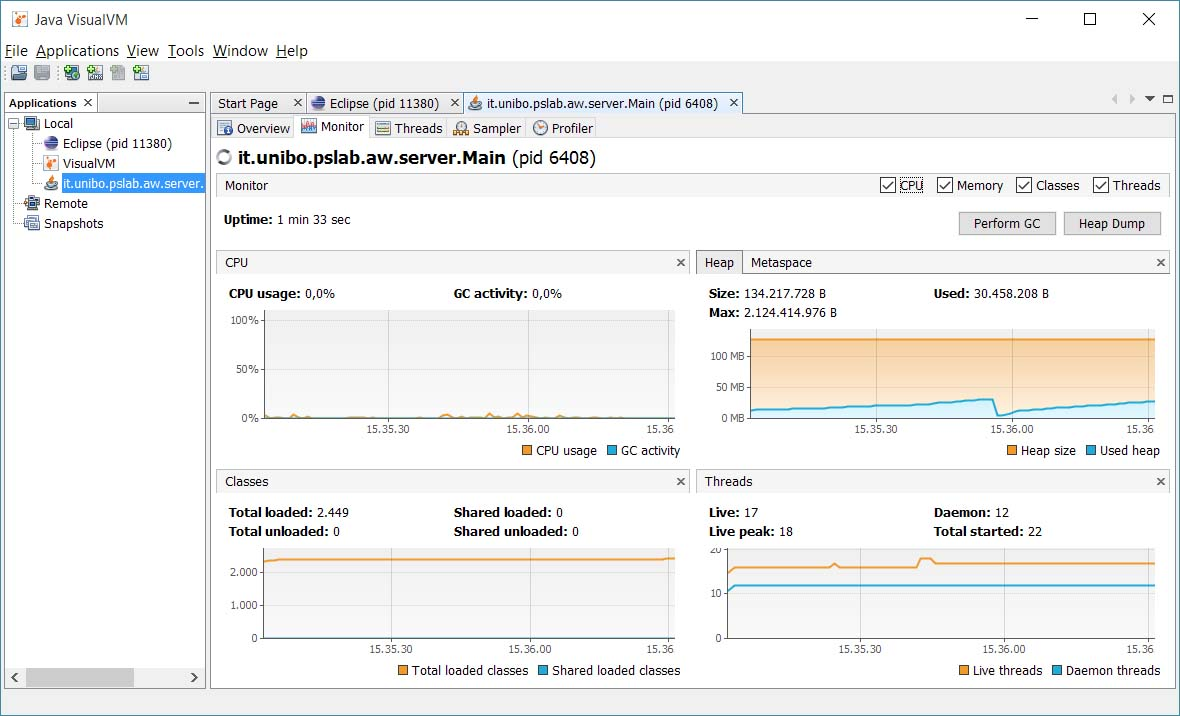
\includegraphics[width=0.99\textwidth]{img/jvisualvm-1}
\end{frame}

\begin{frame}{VisualVM - Threads Status}
\centering
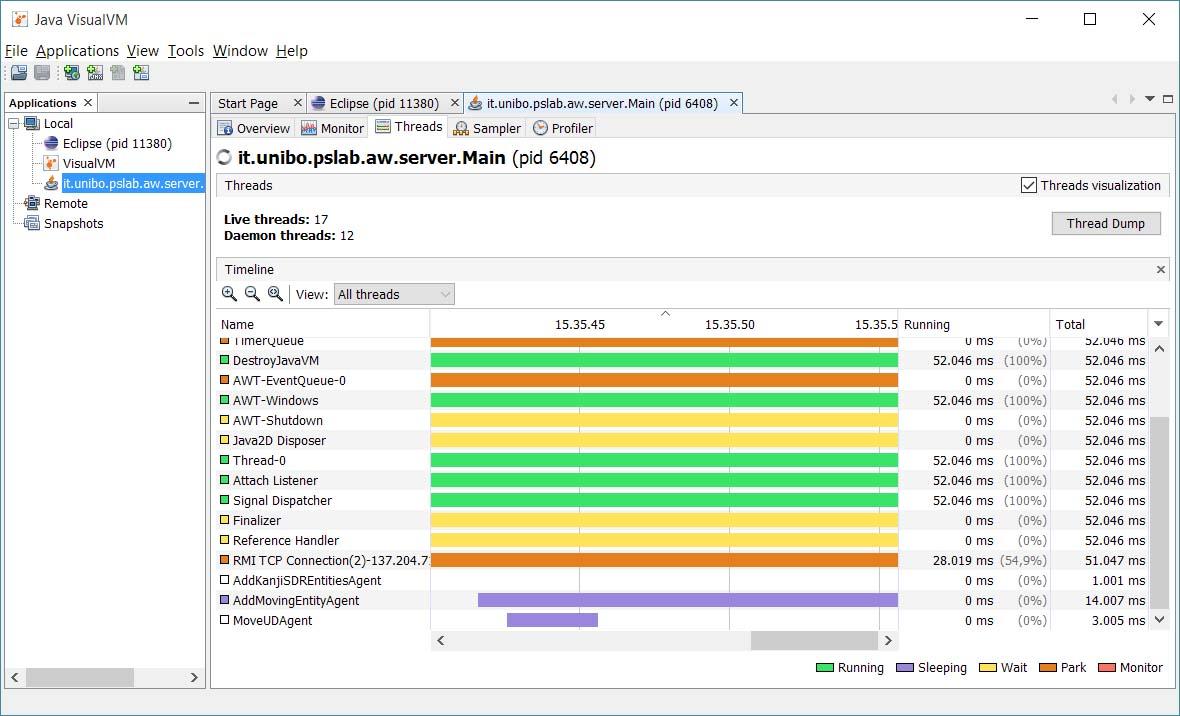
\includegraphics[width=0.99\textwidth]{img/jvisualvm-2}
\end{frame}

\begin{frame}{VisualVM - Thread Dump Example}
\centering
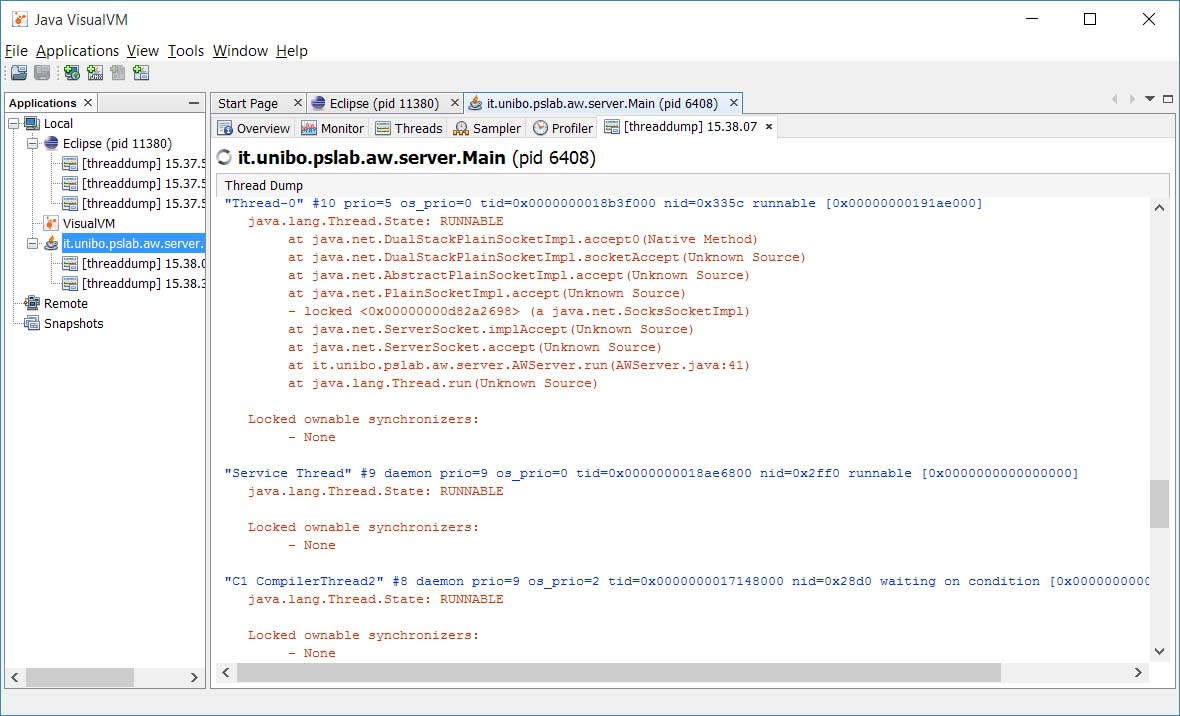
\includegraphics[width=0.99\textwidth]{img/jvisualvm-3}
\end{frame}

\end{document}
